\documentclass[twocolumn]{aastex6}
\usepackage{natbib}
\bibliographystyle{aasjournal}
\usepackage{graphicx}
\usepackage{amsmath}

\def \lya {Ly$\alpha$ }
\def \mkms {{\rm \; km\;s^{-1}}}
\def \msunperyr {{\; M_{\odot}\rm \;yr^{-1}}}

\begin{document}
\title{A VLT/FORS2 Narrowband Imaging Search for \ion{Mg}{2} Emission Around $\lowercase{z}\sim0.7$ Galaxies }
\author{Ryan Rickards Vaught \altaffilmark{1}, Kate H. R. Rubin \altaffilmark{1}, Fabrizio Arrigoni Battaia \altaffilmark{2},  Joseph Hennawi, J. Xavier Prochaska}

\altaffiltext{1}{San Diego State University 5500 Campanile Dr, San Diego, CA 92182}
 \altaffiltext{2}{Max-Planck-Institut fur Astronomie, Konigstuhl 17, D- 69117 Heidelberg, Germany}

\begin{abstract}
Galactic-scale outflows are thought to be the primary mechanism in the removal of cool gas in star-forming galaxies. 
%
Presently, the mass and energy of these flows remain poorly constrained.
%
One way to better constrain these parameters is to measure the spatial extent of the outflow; however, measuring the spatial extent of such outflows via spectral methods has been traditionally very difficult due to the faintness of emission lines tracing outflowing material. 
%
We present VLT/FORS2 narrowband imaging of 5 star forming galaxies at redshift $z=0.67-0.69$ in the GOODS-S field as part of an effort to spatially resolve large-scale outflows traced by \ion{Mg}{2} emission. 
%
Previous spectra of this sample have already revealed winds traced by \ion{Mg}{2} absorption. 
%
At our sample redshift, the \ion{Mg}{2} emission lines fall exactly within the FORS2 HeII+47 and HeII/3000+48 interference filters.
%
The total integration time of 10 hrs obtained in each filter permits the analysis of the flow surface brightness and extent on scales over which \ion{Mg}{2} is typically detected in absorption (i.e., projected distances $> 100$ kpc). 
%
Such measurements can provide stronger constraints on the mass and energy of feedback, helping to advance our understanding of the processes regulating galaxy evolution up to $z=1$. 
\end{abstract}

\maketitle

\section{Introduction}
Galactic scale outflows are considered to be a main driver of galaxy evolution, as they provide a means to transport cool gas away from star forming regions out to the intergalactic medium. 
%
%
In other words, this removal of cool gas carries away the necessary fuel that is required for stellar formation. 
%
%
Even though outflows play a critical role in the star formation rates and mass of the host galaxy \citep{Werk_2014}, the physical production mechanism that powers these outflows remains uncertain.
%
%
Despite the uncertainty, some possible mechanics have been proposed by theoretical studies that include thermal pressure from core collapse supernova, radiation pressure from starbursts and finally cosmic ray pressure \citep{Sugahara_2017,Larson_1974,Chevalier_1985,Springel_2003}. 
%
%
An accurate picture of what types of galaxies host outflows comes from numerous spectroscopic studies(authors), as outflows are detected by measuring the blueshift of absorption transitions with respect to the host galaxy systematic velocities.
%
%
Spectroscopy of galaxies from low to high redshifts and over a wide range of star formation rates have revealed outflows in galaxies which host large concentrations of massive stars (e.g., \cite{Rubin_2014} Martin 2012). 
%

% New Paragraph
One common practice in detecting the presence of gas in distant galaxies has been to spectroscopically probe galactic halos along background quasar sight lines and down-the-barrel observations.
%
With temperatures of the cool halo gas component on the order of $10^4\ K$, the gas can be traced by the absorption of metals such \ion{Mg}{2}, Fe and others \citep{Bordoloi_2011, Bergeron_1986}. 
%
Nonetheless, this method is weak in constraining the overall radial profile, extent and morphology of the outflow. 
%
It follows from these weak constraints that estimates of mass and energy loss are left uncertain by at least two order of magnitude \citep{Rubin_2014}. 

%%%% KHRR
\begin{itemize}
\item One novel way of developing these constraints is to trace the extent of winds in emission

\item This has been done in the optical (in H$\alpha$, [\ion{O}{3}]) for nearby starbursts -- these transitions trace a warm, shock-heated phase

\item In a study by \cite{Rubin_2011} strong \ion{Mg}{2} emission with a P-Cygni line profile was observed in the GOODS-N galaxy TKRS 4389. A proposed production mechanism for the observed \ion{Mg}{2} emission is photon scattering.

\item This latter mechanism makes it possible to study winds in emission beyond the local universe

\item Summary of experiment: in this paper, we present the first narrowband imaging of \ion{Mg}{2} line emission in a sample of five distant ($z\sim0.7$) star-forming galaxies.  State the measurement we're making (SB limit, 2D absorption morphology).

\item Roadmap of paper sections for the reader.

\end{itemize}
%%%% end KHRR


\section{Observations and Data Reduction}

%%%% KHRR
\subsection{Sample Selection}

Our target galaxies were selected from a Keck/LRIS survey of UV absorption lines in $\approx 100$ objects having redshifts $0.3< z < 1.4$ and $B_{AB}< 23$ in fields with deep \emph{HST}/ACS imaging \citep{Rubin_2014}.  In particular, this parent survey targeted galaxies in a total of nine Keck/LRIS pointings located in both of the GOODS fields \citep{Giavalisco2004} and the AEGIS survey field (the Extended Groth Strip; \cite{Davis2007}).  In inspecting the redshift distribution of the portion of this sample observable from the Southern Hemisphere, we uncovered a narrow peak of nine galaxies in the interval $0.66 < z < 0.68$.  This peak is in fact the global maximum of the distribution, as all other bins of width $\Delta z = 0.02$ have at most four galaxies.  Moreover, there are two narrow interference filters available on VLT/FORS2 centered at $\lambda \sim 468.4$ and 472.6 nm which cover the \ion{Mg}{2} $\lambda \lambda 2796, 2803$ transition in precisely this redshift interval.  We selected our final sample of five of these galaxies at $0.66 < z < 0.68$ to be close on the sky such that they could be imaged in a single $7\arcmin \times 7\arcmin$ FORS2 pointing.  

The absorption line modeling presented in \cite{Rubin_2014} indicates that these five galaxies are driving strong outflows traced by \ion{Mg}{2}  with velocities $\sim150-420\mkms$ and equivalent widths $\sim 2-3$ \AA.  Modeling of the galaxy broad-band spectral energy distributions obtained from multiwavelength ancillary imaging data yields star formation rates (SFR) ranging from $\sim4$ to $40\msunperyr$ and stellar masses in the range $\log M_*/M_{\odot}\sim 9.9-11.0$.  These properties, as well as precise target coordinates, are listed in Table~\ref{tab:prop}.  \emph{HST}/ACS images of the galaxy sample are shown in 
Figure~\ref{fig.hstims}.  The Keck/LRIS spectroscopy of this sample published in \cite{Rubin_2014} is shown in Figure~\ref{fig:spec_images}.



%%%%

%
%The  sample is fortuitously distributed on the sky such that it can be imaged in a single FORS2 pointing.

\subsection{VLT/FORS2 Observations}
% New Paragraph
The data were taken in service-mode using the FORS2 instrument on the VLT 8.2m telescope Antu between October 2012 and February 2013. 
%
We used two narrowband filters, HeII+47 and HeII/3000+48, that have peak transmission at wavelengths that correspond to the \ion{Mg}{2} doublet lines at our sample redshift of $z\approx 0.7$ (see Table \ref{tab:filters}).
%%%% KHRR
[{\bf This is demonstrated nicely in Figure~\ref{fig:spec_images}, so I think we should explain it fully and refer to it here.}]
%%%%

%
The FORS2 has a pixel scale of $0.25''$ pixel$^{-1}$ and a field of view of $7'\times7'$.
%
Summing the individual exposure times for each image results in a combined exposure time of $10.0$ hours each for the HeII+47 and HeII/3000+48 filters.
%
Our observations were carried out under photometric and thin cloud conditions (program ID: 090.A-0427A).
%%%% KHRR
[{\bf Explain seeing conditions here and refer to Figure~\ref{fig.seeing}.  You should also explain that the data were taken with three pointings offset by XXX arcmin somewhere in this subsection.}]
%%%%

\begin{figure*}[!ht]
\centering
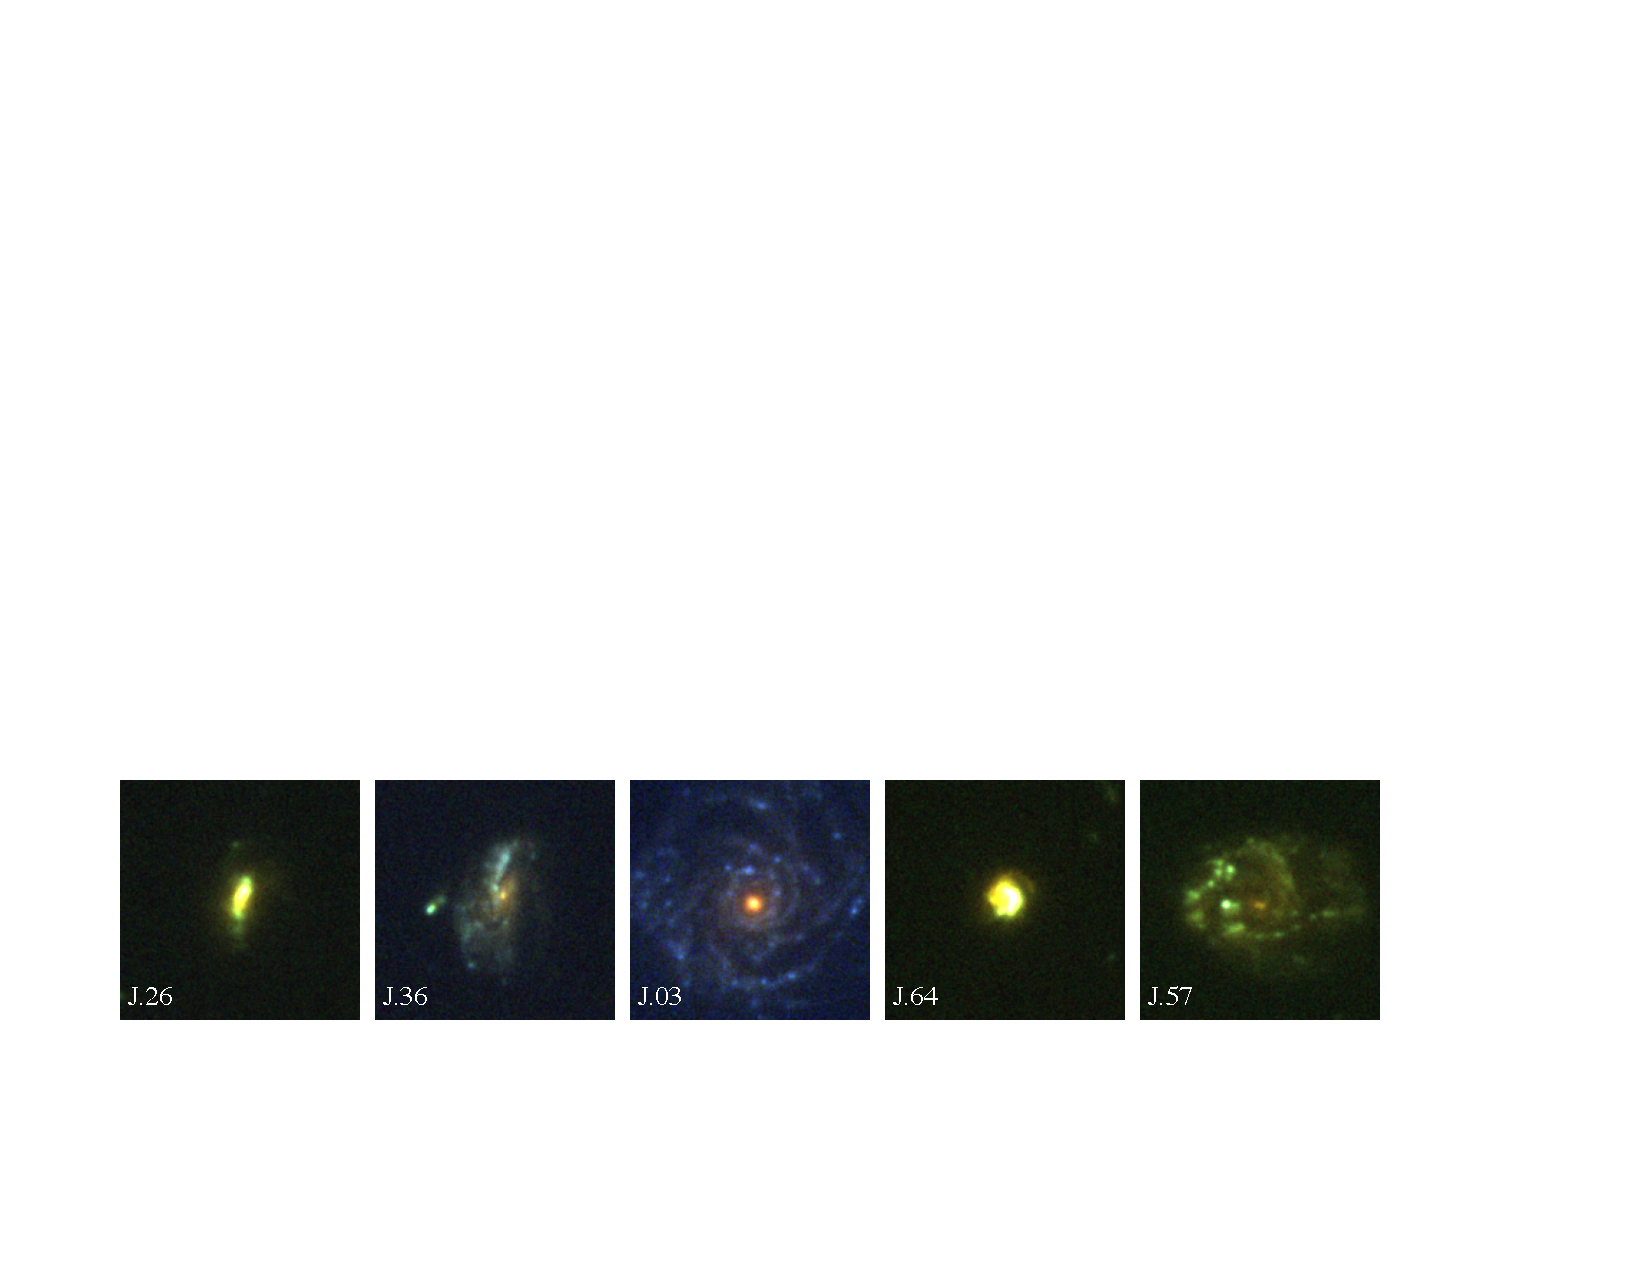
\includegraphics[scale=.75,trim=50 100 100 350,clip=]{../Figures/fors2_color_imstamps.pdf}
\caption{Color imaging of our sample galaxies in the \emph{HST}/ACS F435W, F606W, and F775W filters obtained as part of the GOODS survey \citep{Giavalisco2004}.
%From Top Left to Right Bottom: J033230.03, J033230.64, J033225.26, J033231.36, J033230.57.
Each image is $5\arcsec\times5\arcsec$.
%%% Reminder to KHRR: made with ~/Research/MgII/paper_mgii/Paper2/Analysis/figpro/vaught2017_make_justcolorims.pro
\label{fig.hstims}}
\end{figure*}

\begin{figure*}[!htb]
\centering
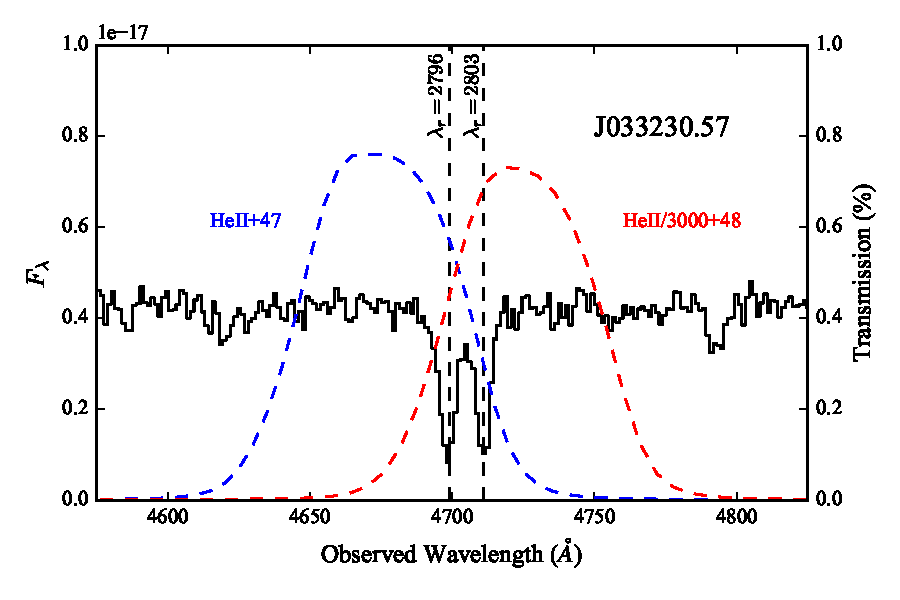
\includegraphics[scale=0.58]{../Figures/filt_57_spectra.pdf}
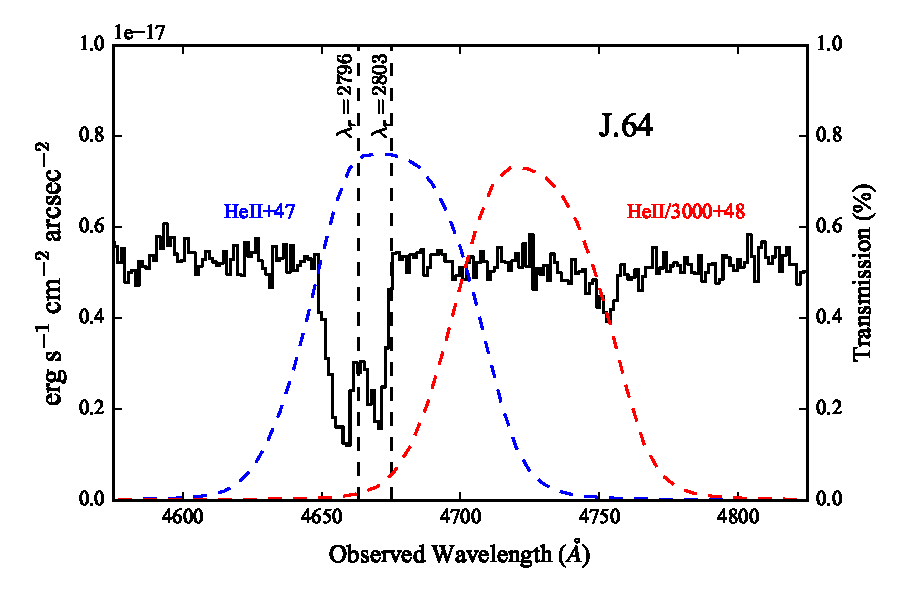
\includegraphics[scale=0.58]{../Figures/filt_64_spectra.pdf}
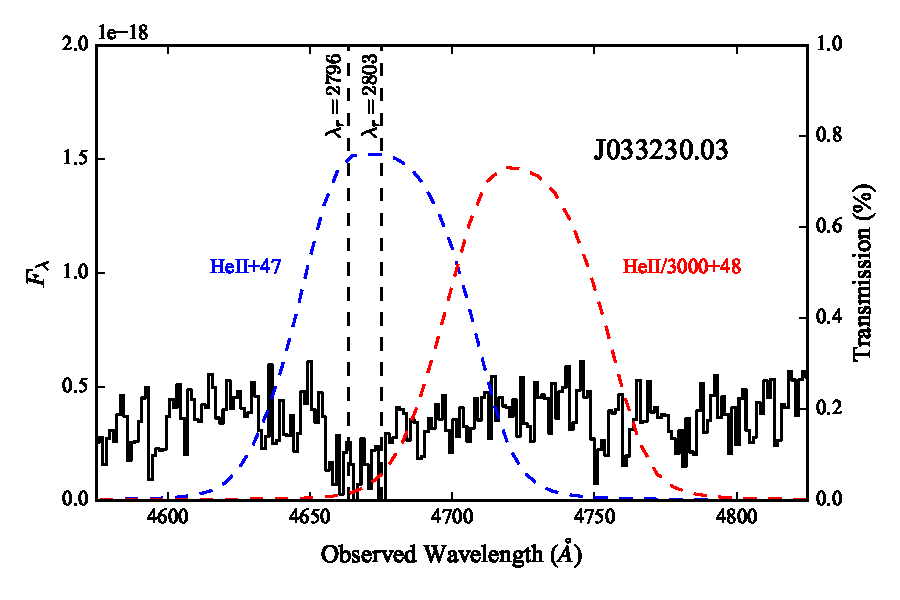
\includegraphics[scale=0.58]{../Figures/filt_03_spectra.pdf}
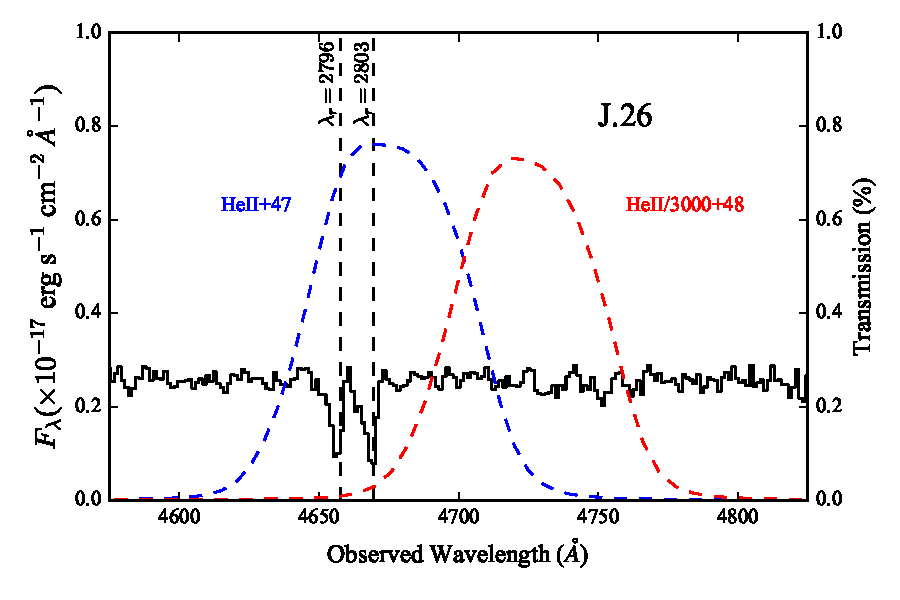
\includegraphics[scale=0.58]{../Figures/filt_26_spectra.pdf}
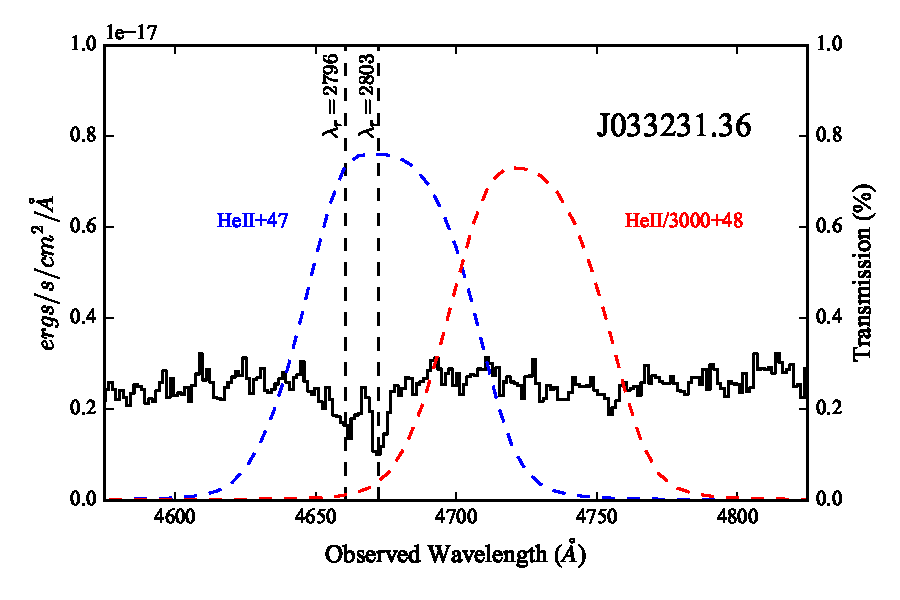
\includegraphics[scale=0.58]{../Figures/filt_36_spectra.pdf}
\caption{KECK/LRIS spectra plotted with the transmission curves of the filters HeII+47 and HeII/3000+48. 
%%%% KHRR
[{\bf Explain the two different y axes, add units to the left-hand y axis, explain what the vertical dashed lines mean.}]
%%%%
The \ion{Mg}{2} doublet falls fortuitously at the central wavelength of the HEII+47 filter. }
\label{fig:spec_images}
\end{figure*}

\begin{figure}[h]
\centering
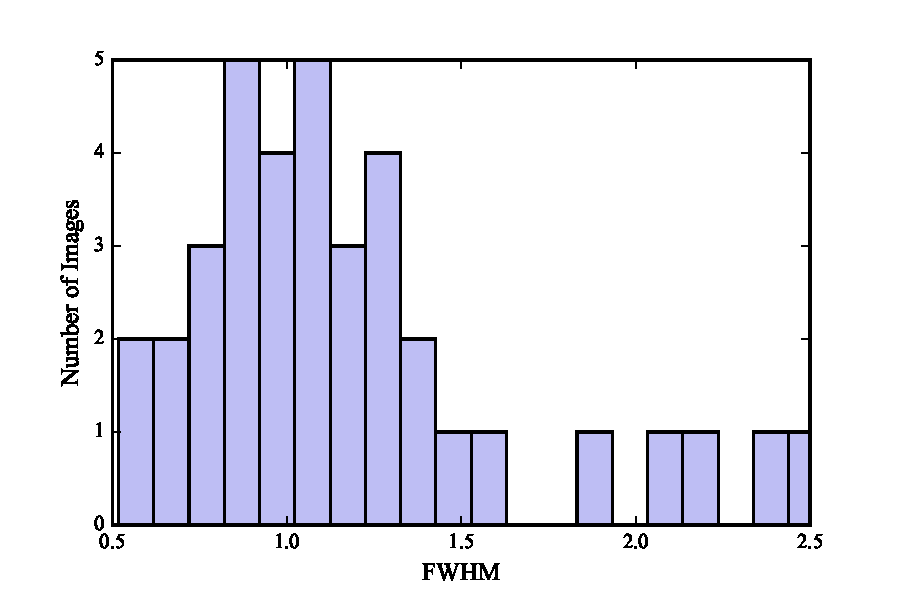
\includegraphics[scale=.55]{../Figures/avg_seeing_HEII.pdf}
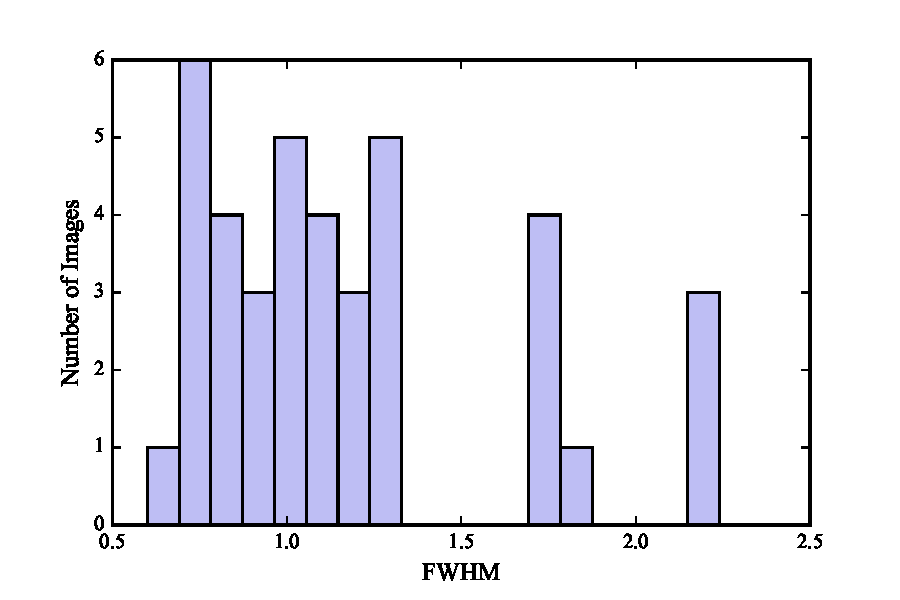
\includegraphics[scale=.55]{../Figures/avg_seeing_HEII3000.pdf}
\caption{  Distribution of seeing conditions for individual exposures comprising our dataset.
%%%% KHRR
\textbf{Top}: Seeing distribution for the XXX HeII+47 images. The median seeing in this filter is $1.03\arcsec$.
\textbf{Bottom}: Same distribution for the XXX HEII/3000+48 images. The median seeing is $1.08\arcsec$. 
%%%%
The seeing conditions were calculated by ESO and were provided in the header of each science image.
\label{fig.seeing}}
\end{figure}



\subsection{Supplemental Keck/LRIS spectra}
In addition to VLT imaging, in the present analysis we utilize galaxy spectra taken from the \cite{Rubin_2014} Keck I Low Resolution Imaging Spectrometer (LRIS) program. A $0.9''$ slit width was used for all slitmasks and the median FWHM resolution for the spectra is 274 km s$^{-1}$ at $\lambda_{\rm rest} \approx$ 2800 \AA\ and $286\mkms$  at $\lambda_{\rm rest}\approx$ 2600 \AA\ (see Figure \ref{fig:spec_images}).

\subsection{Image Reduction}
The data were reduced using custom routines written in \textbf{Python}. 
%%
The images were first corrected by subtracting and removing the overscan region of the CCD. 
%%
Then the images were bias-subtracted and flat-fielded using twilight flats. 
%%
Each individual image was cleaned of cosmic rays and bad pixels by utilizing the L.A. Cosmic algorithm.
%%
 The astrometry solutions were calculated via Astrometry.net \citep{Lang} with a standard deviation in the galaxy coordinates of $\sigma \approx 0.10''$. 

%%
Before image stacking, we ran each frame through \textbf{SExtractor} \citep{Bertin} in order to create a root mean square (RMS) map of each science image.
%%
 These frames, in addition to the science images, are stacked to create a co-added RMS image.
%% New Paragraph
The final stacked images for each filter is obtained using \textbf{SWarp} \citep{Bertin}.
%%
Each individual frame is first sky-subtracted using a background mesh size of 256 pixels which is approximately $64''$. 
%%
We chose the mesh size to be large enough such that the extended emission is not mistakenly subtracted \citep{Battaia_2015}. 
%%
The frame, after background-subtraction, is resampled onto a common astrometric solution using a \textit{Lancosz3} interpolation kernel. 
%%
The images are median-combined in order to increase the signal-to-noise of any \ion{Mg}{2} emission. \textbf{SWarp} is also configured to produce RMS weight maps from our \textbf{SExtractor} weighted images.  

%%%% KHRR
Our final stacked images in each filter are shown in Figure~\ref{fig:stacked_image} with the target galaxies indicated.  
%Once image stacking was done, we were left with two images to perform photometry on. One image contains only continuum photons, while the other one contains continuum + \ion{Mg}{2} photons.  (see Figure \ref{fig:stacked_image}). 
%%%%
One side effect from stacking is that the east and west borders of each image contain greater noise compared to the center of the image. This is due to the imperfect overlap of the 3 pointings used. However, the sample galaxies are sufficiently distant from these low S/N regions that their photometry is not affected. As a final step, both images are aligned in physical coordinates via the IRAF \textbf{Imalign} command \citep{Tody_1986}.



\begin{table}[h!]
\caption{VLT/FORS2 Observations: Filter and exposure properties of the VLT observations. The width of the transmission curves are calculated by convolving the transmission curve with the total wavelength range of the filter. These values differ slightly from those reported by the European Space Observatory. }
\begin{tabular}{llllll} \hline \hline 
Filter & $\lambda_{eff}$(\AA)\footnote{$\lambda_{eff}$ is the effective wavelength of the filter transmission curve.} & $\lambda_{width}$(\text{\AA})    & $N_{images}$   & $t_{tot}(s)$ & $S$\footnote{S is in units of ergs counts$^{-1}$ cm$^{-2}$ }\smallskip \\ 
& & & & & $\times10^{-17}$ \\ \hline 
HeII  & 4675.21 & 50.11 & 38  & 35,959 & 2.45 \\
HeII/3000 & 4722.46  & 44.82 & 38 &   36,937 & 2.40       \\ \hline
\end{tabular}
\label{tab:filters}
\end{table}

\begin{table*}[t]
\centering
\caption{Properties of 5 galaxies in our sample :  These properties were taken from \cite{Rubin_2014}. All galaxies are at roughly the same redshift. The star formation rates for the sample range from 3.8 to 40.5 solar mass per year. The EW are for the blended components of the \ion{Mg}{2} doublet and were calculated with Eq. \ref{eq:specEW} and the supplemental Keck/LRIS spectra.  
%%%% KHRR
{\bf I think you have updates to these EWs and their errors, correct?}
%%%%
}
\begin{tabular}{lllllll} \hline \hline
Object & R.A. & Dec  & $z$ & SFR($M_{\odot} yr^{-1}$) & $\log{M_{*}/M_{\odot}}$ & EW(\AA) \smallskip      \\ \hline 
J033225.26-      & 03:32:25.26 & -27:45:23.9 & 0.6660 & $9.1_{-3.7}^{+1.3}$& $9.86_{-0.04}^{+0.05}$ & $7.00\pm 0.51$\\ 
274524.0     & &  &  &         \\
J033231.36-      & 03:32:31.35 & -27:47:24.9 &   0.6669 & $10.5_{-1.6}^{+1.7}$ & $10.02_{-0.03}^{+0.03}$&$6.50 \pm 0.51$\\
274725.0      & &  &   &        \\
J033230.03-      & 03:32:30.03 & -27:43:47.2  &   0.6679 & $3.8_{-0}^{+0}$ & $10.98_{-0.0}^{+0.01}$ &$6.44 \pm 0.51$\\
274347.3      & &  &   &        \\
J033229.64-      & 03:32:29.64 & -27:42:42.5 & 0.6671 & $40.5_{-12.1}^{+8.2}$ & $10.30_{-0.03}^{+0.07}$ &$6.70 \pm 0.51$\\
274242.6     & &  &     &      \\
J033230.57-      & 03:32:30.56 & -27:45:18.2 &   0.6807  & $12.6_{-2.1}^{+1.7}$ & $10.48_{-0.07}^{+0.03}$ &$5.60 \pm 0.52$ \\
274518.2      & &  &  &         \\ \hline 
\end{tabular}

\label{tab:prop}
\end{table*}


\subsection{Absolute Flux Calibration}
We acquired observations of the standard star GD50 from archival ESO calibration imaging
%%%% KHRR
at XXX independent epochs.
%%%% 
From this standard we calculated the atmospheric extinction coefficients to be 0.181 magnitudes for the HeII/3000+48 filter and 0.190 magnitudes for the HeII+47 filter. Since we have imaging of the standard star GD50 in our two filters, and access to GD50's spectral energy distribution (cite!) and each filter's transmission curve through the ESO website, we are able to perform absolute flux calibration using the methods of Jacoby et al. (1990). We first convolve the spectral energy distribution of the standard star, $F(\lambda)$ in ergs sec$^{-1}$ \AA$^{-1}$ cm$^{-2}$, with that of the known transmission curve of the filter, $T_{i}(\lambda)$. This yields $F_i$, the total observable flux in each bandpass filter $i$ with units of ergs sec$^{-1}$ cm$^{-2}$:
\begin{equation*}
F_{i}=\int F(\lambda)T_{i}(\lambda)d\lambda.
\end{equation*}
It is not uncommon to assume that $F(\lambda)$ is constant over the small width of the filter. However, our filter transmission curves are sampled at $5$\ \AA\ intervals which is the same sampling as the spectral energy distribution of the standard star obtained from the ESO archives. Therefore we calculate the integral numerically.
The system sensitivity, including the defects of the telescope optics and detector response is then given by
\begin{equation*}
S_{i}=\dfrac{F_{i}}{C10^{k_{i}A}},
\end{equation*}\\
where $k_i$ is the extinction in magnitudes per airmass, A is the airmass for each individual exposure, C is the measured count rate of the standard star and $S$ is in units of ergs counts$^{-1}$ cm$^{-2}$. Before image co-addition, each science image is corrected for atmospheric extinction by multiplying each frame by $10^{k_{i}A}$. Next, the image is divided by the exposure time, effectively putting the image in units of counts per sec. After co-addition, the images are then multiplied by the appropriate sensitivity factor $S_{i}$. This puts the final images in the appropriate flux units ergs sec $^{-1}$ cm$^{-2}$.

\begin{figure*}[ht!]
\centering
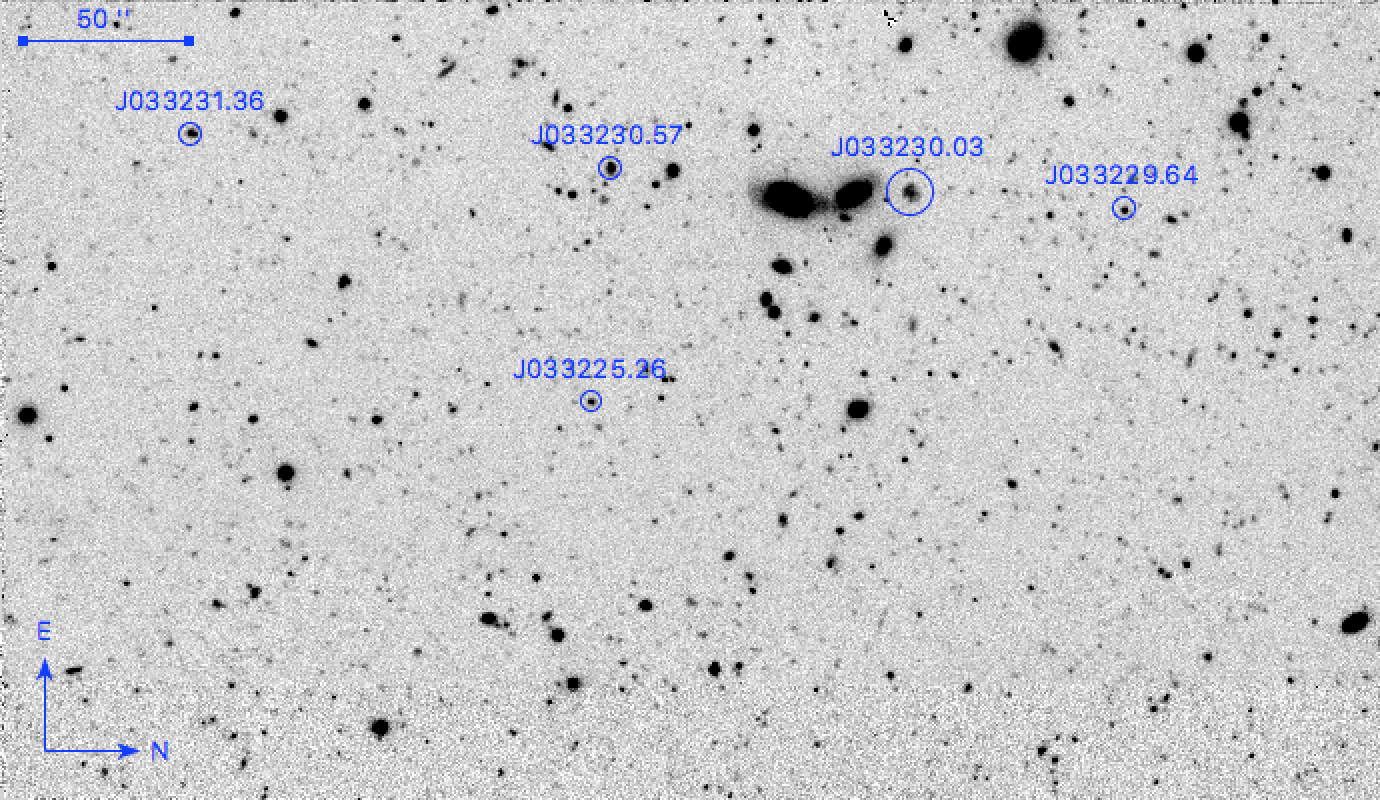
\includegraphics[scale=.61]{../Figures/HEII_final.png}
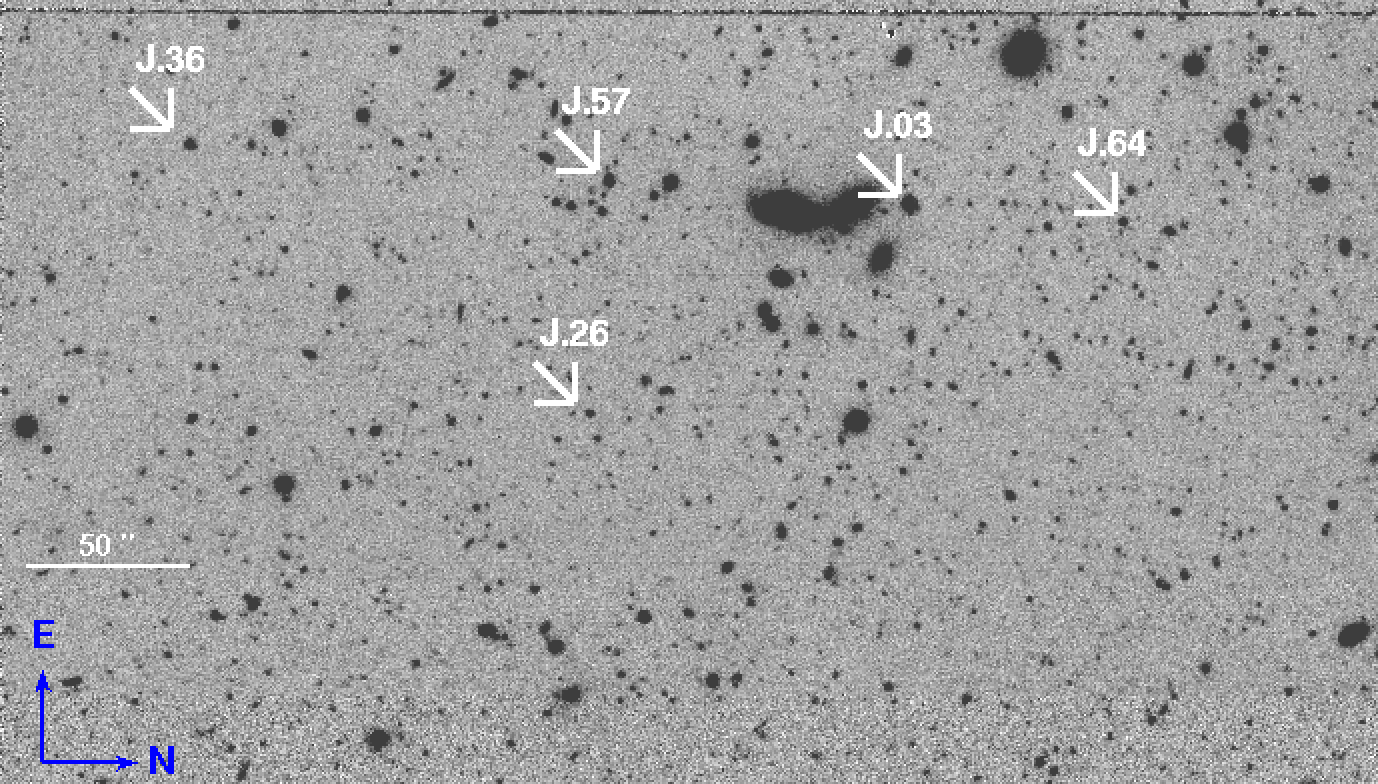
\includegraphics[scale=.61]{../Figures/HEII3000_final.png}
\caption{Top: HeII+47 image after stacking. Bottom: HeII3000+48 image after stacking. 
%%%% KHRR
[{\bf Add total exposure time of each image, specify the total field of view, that east is up and north is to the right, and that the sample galaxies are indicated with blue symbols.  Also, what is the grayscale here?  Are these in counts/sec or in flux units?}]
%%%%
}
\label{fig:stacked_image}
\end{figure*}

\section{Analysis}

%%%% KHRR
 We have two goals for our study: (1) assess the surface brightness of line emission in the \ion{Mg}{2} transition in and around each target galaxy; and (2) spatially resolve the morphology of the strong \ion{Mg}{2} absorption observed against the galaxy continua.  To reach the both of these goals, we must perform accurate subtraction of the continuum flux of each object from the filter covering the targeted line emission.  
For four of the five objects in our sample, the HeII+47 image includes both line and continuum emission, and 
the HeII3000+48 image provides a high S/N measurement of the continuum only $\approx30$ \AA\ redward of the line emission in the rest-frame.  We detail our method of continuum subtraction using these data in Section~\ref{subsec.cont_sub} below, and follow with a presentation of the resulting surface brightness profiles (Section~\ref{subsec.sb}) and EW images (Section~\ref{subsec.ew}).
%%%%


\subsection{Spectral Correction}
With the supplementary spectra from \cite{Rubin_2014}, we can fit the continuum and determine the slope of each galaxy spectrum in order to determine if the spectral slope gives rise to differences in continuum flux between the two filters. We use the interactive fitting routine \textbf{lt\_continuumfit} from the linetools package (Prochaska et al. 2016)\footnote{https://github.com/linetools/linetools} to fit the continuum. By fitting the continuum we are masking the absorption features and making an effectively flat spectrum, which we use as a model. We find the total flux in each filter by convolving the fitted continuum with each filter's transmission curve. Next, we take the ratio of both integrated totals, as the ratio will indicate the scaling factor needed to correct either of the filters. Comparing these ratios between each galaxy, we find that each ratio is effectively the same, within 1/1000 percent, with a value of 1.118. 
%%%% KHRR
[{\bf 1/1000 percent would be 0.00001 -- which seems unrealistically small.}]
%%%%
This value is equal to the ratio between the FWHM of the transmission curves, allowing us to conclude that the slope of the spectrum of each galaxy does not affect the continuum values collected in either filter.

\subsection{Continuum Subtraction}\label{subsec.cont_sub}
To properly continuum-subtract the image taken with the emission filter in excess of the continuum, we follow a prescription given by \cite{Battaia_2015}. 
We first determine the continuum flux density from the off-\ion{Mg}{2} filter,
\begin{equation}
f_{cont}=\frac{F_{cont}}{\Delta \lambda_{cont}},
\end{equation}\\
where $F_{cont}$ and $\Delta \lambda_{cont}$ are the observed flux per pixel of the continuum image per pixel and the transmission FWHM of the continuum filter, respectively. With $f_{cont}$ it is then possible to calculate the flux of any excess emission, $F_{line}$:
\begin{equation}
F_{line}=F_{MgII}-f_{cont} \Delta \lambda_{MgII}
\label{eq:subtraction}
\end{equation}
where $F_{MgII}$ and $\Delta \lambda_{MgII}$ are the observed flux per pixel in the \ion{Mg}{2} filter and the transmission FWHM of the \ion{Mg}{2} filter. The continuum subtracted images of each galaxy are shown in Fig. \ref{fig:stamp_images}.

\begin{figure*}[!htb]
\centering
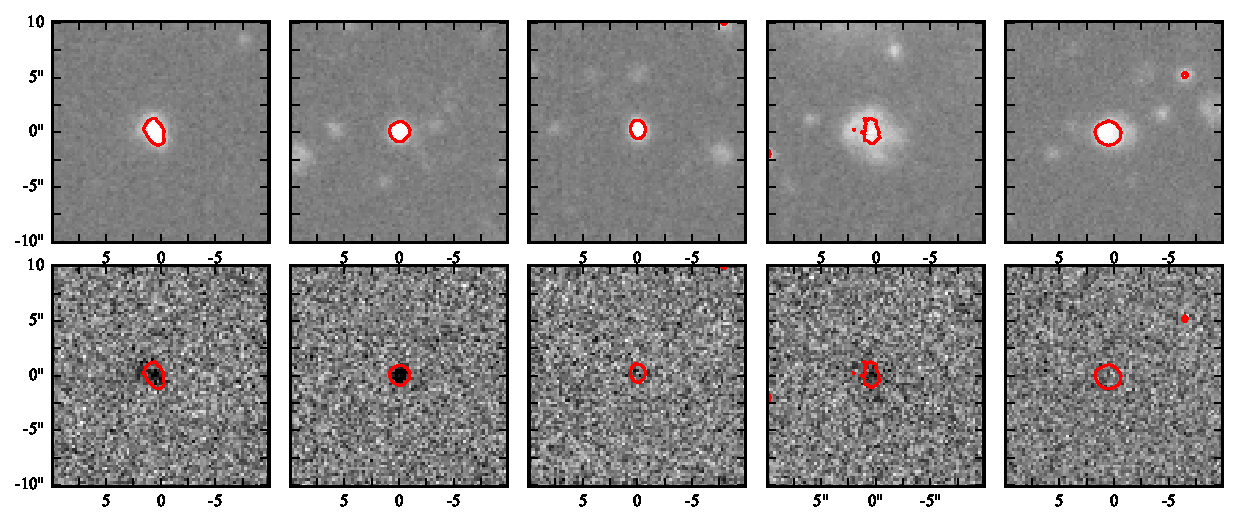
\includegraphics[scale=0.7]{../Figures/stamps.pdf}
\caption{ $10'' \times 10''$ images stamps. Top row: Continuum flux in ergs/s/cm$^2$/arcsec. Bottom row: Continuum subtracted \ion{Mg}{2} flux.  Absorption can be seen in 3 of 5 galaxies. Each stamp is scaled with symmetric limits around 0.
%%%% KHRR
[{\bf Explain what the red contours are, and add color bar if possible.  Also, label axes with ``arcsec''.  Would be nice to add labels indicating the IDs of each galaxy.  Also, I expect Joe will ask for a $\chi^2$ version of these postage stamps, as in Fabrizio's Fig. 10.}]
%%%%
}
\label{fig:stamp_images}
\end{figure*}

\subsection{Surface Brightness Profiles and Limits}\label{subsec.sb}

In order to test for the presence of \ion{Mg}{2} emission, we perform aperture photometry on the continuum subtracted images using the python library Photutils. We choose apertures
%%%% KHRR
[{\bf I think we may want to replace the word ``apertures'' with ``annuli'' throughout this paragraph and the next -- do you agree?}]
%%%%
 with thickness of 2 pixels or $0.50 ''$, such that, $r_{inner}=r_{outer}-2$ (in pixels). Each aperture is centered on the flux-weighted centroid of the galaxy. We also consider an aperture with an inner radius of 24 pixels ($6''$) and outer radius of 30 pixels ($7.5''$) in order to increase our sensitivity to extended emission. Dividing the summed flux in each aperture by the area in arcsecs we produced surface brightness (SB) profiles for each galaxy. 

The error bars are determined from a weight image produced by \textbf{SWarp}. The weight image is converted to an RMS image by taking the square root of the inverse weight. We then place apertures that are identical to the apertures used to find the SB profiles for each galaxy. To calculate the variance inside each aperture, we sum the RMS pixel values in quadrature, then divide by the area of each aperture. 

To calculate the $3\sigma$ SB detection limit in each filter, we first masked out all the sources, their associated extended halos, and edge noise in both the HE+47 and HE/3000+48 images. We then calculated the root-mean-square of the background in randomly placed apertures with radii that matched the aperture radii used to measure the SB of the galaxies. The RMS values were then converted into SB in 1 square arcsec apertures. 
%%%% KHRR
[{\bf Up to here in this paragraph, it seems like the word ``apertures'' should stay -- but do you mean annuli below?  That is, are you calculating a SB limit for a doughnut-shaped annulus?  (And if not, doesn't the absorption screw with the measurement a bit?)}]
%%%%
These values are calculated to be $5.120\times10^{-18}$ ergs sec $^{-1}$ cm$^{-2}$ arcsec$^2$ and $4.154\times10^{-18} $ ergs sec $^{-1}$ cm$^{-2}$ arcsec$^2$ in the HeII/3000 and HeII filters, respectively. We repeated the above procedure to obtain SB limits for the set of continuum-subtracted images: we calculated the root-mean-square of the flux inside the largest aperture. We determined the 3$\sigma$ SB limits to be $2.09\times10^{-18}$ergs sec $^{-1}$ cm$^{-2}$ arcsec$^2$ and $1.87\times10^{-18}$ ergs sec $^{-1}$ cm$^{-2}$ arcsec$^2$ for the HeII - HeII/3000 combination and the HeII/3000 - HeII combination. 

\subsection{Equivalent Widths}\label{subsec.ew}
Here we derive an expression to calculate the equivalent width (EW) of any absorption or emission features observed in our narrow-band imaging. Starting from the expression for EW used in the context of spectroscopy,
\begin{equation}
EW=\int (1-\frac{f_{line}}{f_{cont}})d\lambda
\label{eq:specEW}
\end{equation}
we begin by dividing Eq \ref{eq:subtraction} by the flux density of the continuum and the FWHM of the on-line filter,
\begin{equation}
\frac{F_{line}}{f_{cont}\Delta \lambda_{MgII}}=\frac{F_{MgII}}{f_{cont}\Delta \lambda_{MgII}}- 1.
\end{equation}
Next, we rearrange the above expression such that we produce the argument of the integrand in Eq. \ref{eq:specEW} on the RHS,
\begin{equation}
-\frac{F_{line}}{f_{cont}\Delta \lambda_{MgII}}=1-\frac{f_{MgII}}{f_{cont}}.
\end{equation}
We then approximate the integration in Eq. \ref{eq:specEW} by multiplying the integrand above by the FWHM of the on-line filter $d\lambda=\Delta \lambda_{MgII},$
\begin{equation}
-\frac{F_{line}}{f_{cont}}=(1-\frac{f_{MgII}}{f_{cont}})\Delta \lambda_{MgII};
\end{equation}
such that
\begin{equation}
EW=-\frac{F_{line}}{f_{cont}}.
\end{equation}

Using the above equation along with the continuum and continuum subtracted images, we produce images of the EW. 
%%%% KHRR
These images are displayed in Figure~\ref{fig:ew_images} within the 1$\sigma$ SB contours of the corresponding continuum images.
%%%%
%The EW are displayed inside a 1$\sigma$ SB contour of continuum flux.
 Outside this contour, the EWs become poorly constrained due to the lack of S/N in the continuum.  %, see Figure \ref{fig:ew_images}. 

\section{Results}
In this section we present the results from the continuum-subtraction of the off-line continuum filter to that of the on-line emission filter. 

\subsection{Limits on the \ion{Mg}{2} emission}
The surface brightness profiles presented in Fig. \ref{fig:sb_profiles} do not exhibit any signs of extended \ion{Mg}{2} emission. Previous constraints on the brightness of any possible emission are given by  \cite{Rubin_2011}. In this work the authors studied emission in a starburst galaxy at $z=0.69$ with a star formation rate of 80 $M_{\odot} yr^{-1}$. In a two-dimensional Keck/LRIS spectrum of this galaxy, they measured fluxes of $4.04 \pm 0.4$ to $8.0\pm 0.4$ $10^{-18}$ergs sec $^{-1}$ cm$^{-2}$  above and below the continuum region of the 2D spectra at $\lambda 2796$. Converting the 3$\sigma$ detection limit of our continuum-subtracted \ion{Mg}{2} image into flux units, we report the \ion{Mg}{2} emission 3$\sigma$ limits as 5.37 $10^{-18}$ergs sec $^{-1}$ cm$^{-2}$. 
%%%% KHRR
[{\bf How do you convert to flux units here?  What size are you assuming?}]
%%%%
Comparing our SB limit to previously reported values, it should be possible to detect the emission of this particular starburst galaxy in our FORS2 imaging.

\subsection{\ion{Mg}{2} absorption in the line-profile}
Although we do not measure any extended \ion{Mg}{2} emission, we do observe a decrement of flux in the galaxy continua measured in the \ion{Mg}{2} filter in 3 galaxies out of the 5 galaxy sample. In the following section we discuss the absorption in each of these three galaxies, as well as our null detections.

We first discuss the case of a null detection of \ion{Mg}{2} absorption. The galaxy J033230.57 at a redshift of $z=0.6807$ is the most redshifted galaxy of the sample. This galaxy shows no significant flux decrement in the \ion{Mg}{2} filter. Examining Figure \ref{fig:spec_images}, we can see that there should not be any absorption measured in J033230.57, as the absorption profile in the spectrum appears both in the HeII and HeII/3000 filter. This is a good test of our flux calibration, as it appears that there are no hints of systematic false absorption signatures.

We have a second case in which we detect quite strong absorption. The galaxy J033230.64 exhibits a maximum flux decrement of roughly $4\times10^{-18}$ ergs sec $^{-1}$ cm$^{-2}$ arcsec$^{-1}$ due to \ion{Mg}{2} absorption. The absorption is exhibited predominantly within the $1\sigma$ SB outline of the continuum. The mean value of the EW in all the pixels within the $1\sigma$ SB outline of this galaxy is $7.88 \pm 0.403$ \AA, which is relatively close to the EW calculated from the spectra, $6.70 \pm 0.51$\ \AA. We expect that the small difference is due to the collecting area of the different methods. We calculate the EW inside a $1\sigma$ region around the core of the galaxy
%%%% KHRR
[{\bf which is approximately how big in arcsec?}]
%%%%
, whereas the spectrum is obtained using a $0.9''$ slit width. In addition, further inspecting the distribution of the EW over the pixels, there are two outlier values of EW$\approx 20$ \AA\ that are influencing the mean value.

The next galaxy that shows a decrement of flux from \ion{Mg}{2} absorption is J033231.36. The \ion{Mg}{2} absorption spills outside the $1\sigma$ continuum flux contour, however a significant amount lies within our $1\sigma$ significant detection. The mean value of the EW of this galaxy is $6.91 \pm 0.560$ \AA, and is in good agreement with the EW calculated from the Keck/LRIS spectra, $6.50 \pm 0.51$ \AA. Again, inspection of the distribution of the EW over the pixels reveals a possible outlier of an EW$\approx 20$\ \AA.


\begin{figure*}
\centering
\gridline{\fig{../Figures/J033225_26.pdf}{0.5\textwidth}{(J033225.26)}
          \fig{../Figures/J033230_03.pdf}{0.5\textwidth}{(J033230.03)}}
\gridline{\fig{../Figures/J033230_64.pdf}{0.5\textwidth}{(J033230.64)}
          \fig{../Figures/J033231_36.pdf}{0.5\textwidth}{(J033231.36)}}
\caption{Surface brightness profiles for galaxies that exhibit flux decrements from \ion{Mg}{2} absorption. Photometry was performed with circular apertures with increasing inner and outer radii. The error bars are determined from a SWarp RMS map.
%%%% KHRR
[{\bf Explain what each color means.  And it would be great if you could add your measurement for the extra-thick annulus here -- perhaps with a different symbol.  Actually... didn't you show me a newer version of these figures recently?}]
%%%%
}
\label{fig:sb_profiles}
\end{figure*}




\begin{figure*}[h!]
\centering
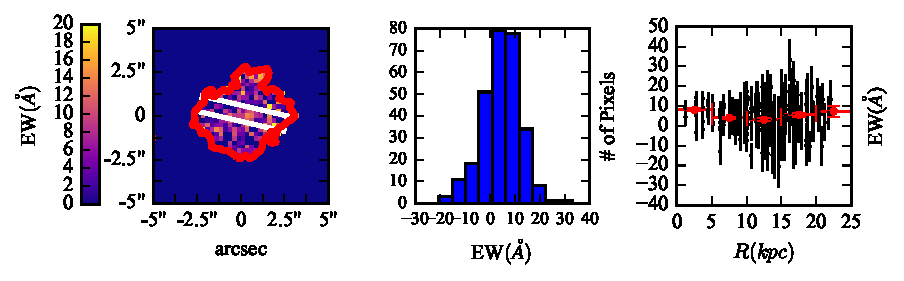
\includegraphics[scale=.58]{../Figures/J03EW.pdf}
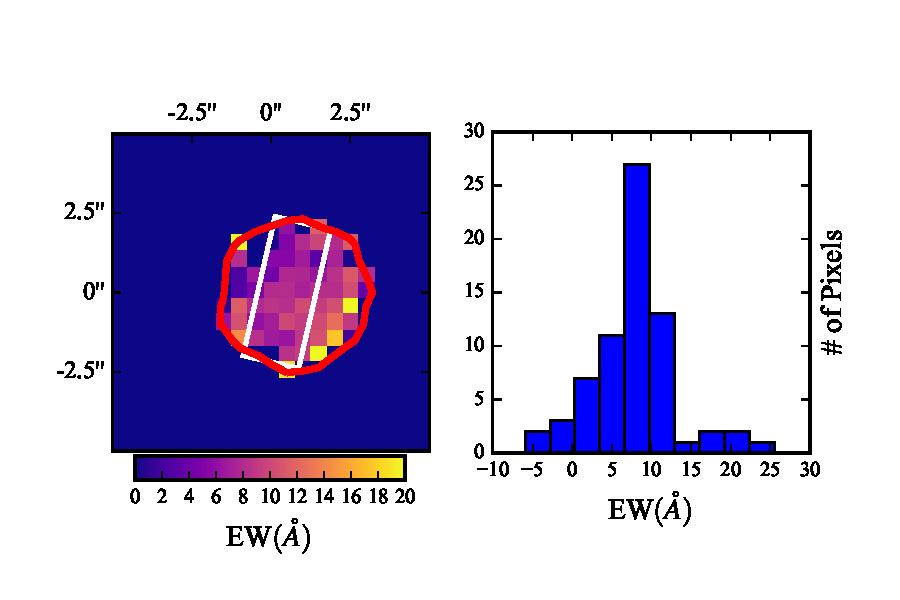
\includegraphics[scale=.58]{../Figures/J64EW.pdf}
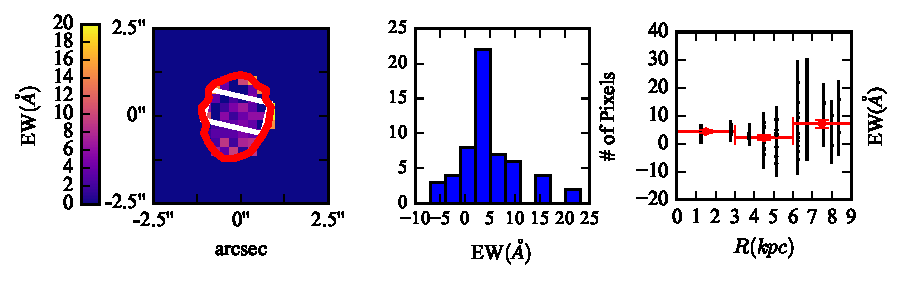
\includegraphics[scale=.58]{../Figures/J26EW.pdf}
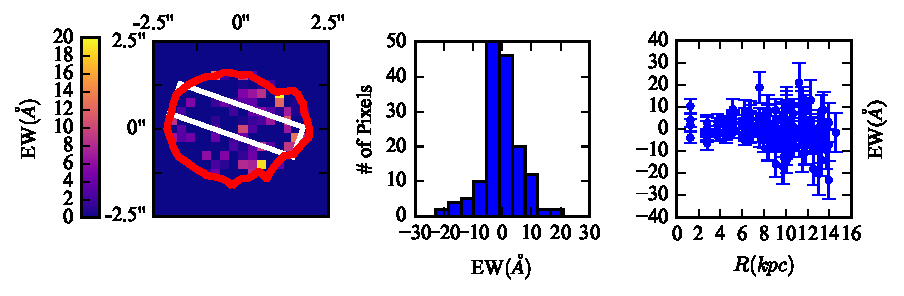
\includegraphics[scale=.58]{../Figures/J57EW.pdf}
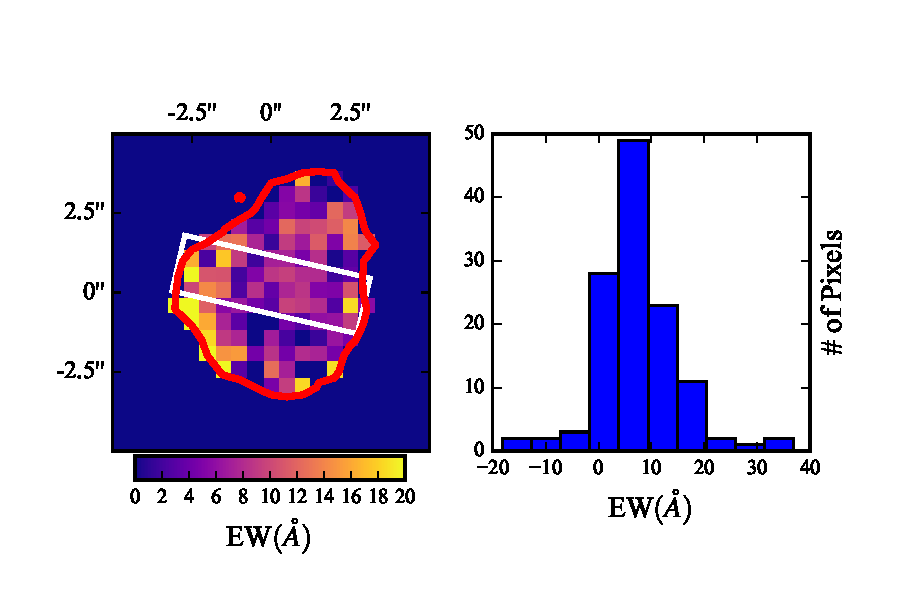
\includegraphics[scale=.58]{../Figures/J36EW.pdf}
\caption{ Plots of the distribution of equivalent widths inside a $1\sigma$ continuum flux outline. 
%%%% KHRR
[{\bf Are these white contours the same as the red contours in Fig. 5?  If so, you should state this.}]
%%%%
}
\label{fig:ew_images}
\end{figure*}

\section{Discussion}

%%%% KHRR
\begin{itemize}

\item Plot of SFR or $M_*$ vs.\ \ion{Mg}{2} SB for this sample, plus \cite{Rubin_2011} and \cite{Martin_2013} galaxies?  (Might be able to include an SB from \cite{Erb_2012} as well.)

\item Construct simple model to investigate effects of seeing / absorption signal on our sensitivity to extended emission?

\item Can we comment on wind morphology / isotropy?  How does absorption EW compare with emission EW implied by our SB limit?

\end{itemize}
%%%%

\section{Conclusion}
We presented the results of a narrowband imaging search for \ion{Mg}{2} emission in a sample of GOODS-S galaxies at a redshift of $z \approx 0.70$. Although we were unable to detect any measurable amount of \ion{Mg}{2} emission, We were able to detect a non-trivial amount of \ion{Mg}{2} absorption in 3 of our 5 galaxy sample. Our images, which are effective in creating absorption maps, were used to calculate the EW of absorption inside a $1\sigma$ continuum contour. 
\bibliography{references2017}






\end{document}